\documentclass[border=4pt]{standalone}
\usepackage[utf8]{inputenc}
\usepackage[T1]{fontenc}
\usepackage{amsmath,amssymb}
\usepackage{tikz}
\usetikzlibrary{arrows.meta,positioning,calc,3d}
\usepackage{pgfplots}
\pgfplotsset{compat=1.18}
% Se compila desde la carpeta docs/: las rutas de datos son relativas a ella.
\begin{document}
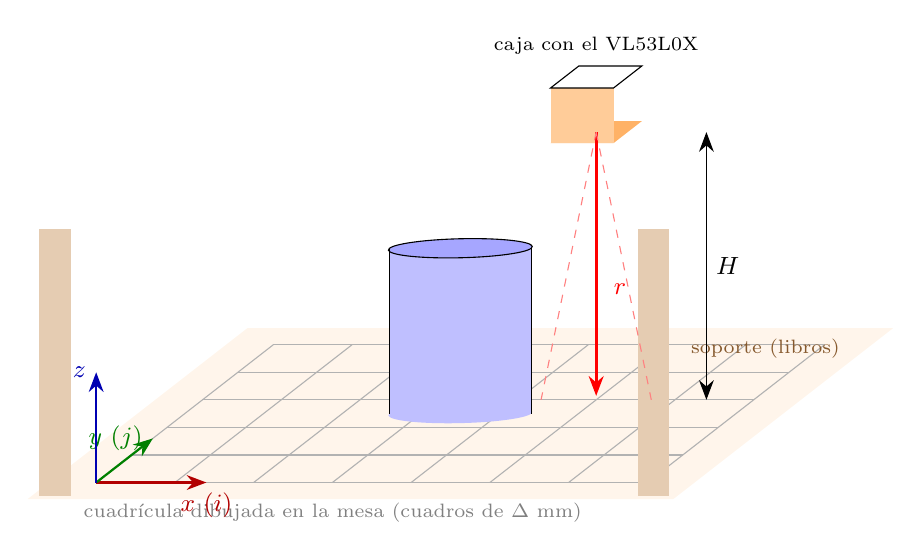
\begin{tikzpicture}[x={(1cm,0cm)}, y={(0.45cm,0.35cm)}, z={(0cm,1cm)}, >={Stealth[length=2.5mm]}, font=\small]
% mesa y cuadrícula
\fill[orange!8] (-0.6,-0.6,0) -- (7.6,-0.6,0) -- (7.6,5.6,0) -- (-0.6,5.6,0) -- cycle;
\foreach \i in {0,...,7} \draw[gray!60] (\i,0,0) -- (\i,5,0);
\foreach \j in {0,...,5} \draw[gray!60] (0,\j,0) -- (7,\j,0);
\node[gray, font=\scriptsize] at (3.5,-1.1,0) {cuadrícula dibujada en la mesa (cuadros de $\Delta$ mm)};
% objeto: un cilindro (taza)
\fill[blue!25] (3.5,2.5,0) ellipse[x radius=0.9, y radius=0.35];
\fill[blue!25] (2.6,2.5,0) rectangle (4.4,2.5,2.1);
\fill[blue!35] (3.5,2.5,2.1) ellipse[x radius=0.9, y radius=0.35];
\draw (2.6,2.5,0) -- (2.6,2.5,2.1) (4.4,2.5,0) -- (4.4,2.5,2.1);
\draw (3.5,2.5,2.1) ellipse[x radius=0.9, y radius=0.35];
% rieles (pilas de libros)
\fill[brown!40] (-0.5,-0.5,0) rectangle (-0.1,-0.5,3.4);
\fill[brown!40] (7.1,-0.5,0) rectangle (7.5,-0.5,3.4);
\node[brown!70!black, font=\scriptsize, align=center] at (8.5,0,1.7) {soporte\ (libros)};
% la caja con el sensor sobre la casilla (5, 3)
\fill[orange!60] (4.6,2.6,3.4) -- (5.4,2.6,3.4) -- (5.4,3.4,3.4) -- (4.6,3.4,3.4) -- cycle;
\fill[orange!40] (4.6,2.6,3.4) -- (5.4,2.6,3.4) -- (5.4,2.6,4.1) -- (4.6,2.6,4.1) -- cycle;
\draw (4.6,2.6,4.1) -- (5.4,2.6,4.1) -- (5.4,3.4,4.1) -- (4.6,3.4,4.1) -- cycle;
\node[font=\scriptsize] at (5,3,4.5) {caja con el VL53L0X};
% haz hacia abajo y cono
\draw[red, very thick, ->] (5,3,3.4) -- (5,3,0.05);
\draw[red!50, dashed] (5,3,3.4) -- (4.3,3,0) (5,3,3.4) -- (5.7,3,0);
\node[red, right] at (5.1,3,1.4) {$r$};
% altura H
\draw[<->] (6.4,3,0) -- node[right] {$H$} (6.4,3,3.4);
% ejes
\draw[->, thick, red!70!black] (0,0,0) -- (1.4,0,0) node[below] {$x$ ($i$)};
\draw[->, thick, green!50!black] (0,0,0) -- (0,1.6,0) node[left] {$y$ ($j$)};
\draw[->, thick, blue!70!black] (0,0,0) -- (0,0,1.4) node[left] {$z$};
\end{tikzpicture}
\end{document}
